% ShelfSense weekly reports 3 and 4.
% Paste into the Overleaf main file in place of the empty "\section{Weekly Report 3}" and
% "\section{Weekly Report 4}" headings. Upload the files in figures/ to the Overleaf project and
% add the entries in new_refs.bib to ref.bib. Lines marked \TODO{...} need a team member.

\section{Weekly Report 3}

\subsection{Follow-up from last week}
Status of the targets set in Weekly Report 2:
\begin{enumerate}
  \item \textbf{SKU-110K sample and simulated videos --- Replaced.} We obtained three real phone
  videos of branded beverage fridges in Bangladeshi shops and used them instead of simulated
  video. The SKU-110K download moved to Sprint 4, where it is used to train the detector.
  \item \textbf{Kaggle notebook for Qwen2-VL-2B --- Done.} The notebook runs Qwen2-VL-2B-Instruct
  \cite{wang2024qwen2vl} zero-shot in fp16 on a free Kaggle T4 GPU (Section~\ref{sec:r3-vlm}).
  \item \textbf{Prompts for the audit tasks --- Done.} Five prompts: fridge brand, product brands,
  counts per brand, empty space and price tags, each with a JSON answer format.
  \item \textbf{Evaluation set --- Partly done.} A ground-truth file lists the fridge brand, the
  product brands, empty space and price tags for each video. Per-brand counts and the brands in
  the third video are still unverified, so all numbers below use a draft ground truth.
  \item \textbf{Baseline results and failure cases --- Done.} Two prompt versions were run and
  scored automatically (Tables~\ref{tab:r3-results} and \ref{tab:r3-failures}).
  \item \textbf{Video VLMs in the literature table --- \TODO{status}.}
\end{enumerate}

\subsection{Work narrative of the current week}

\subsubsection{Refined problem: verifiable audits}
Our team's knowledge of Bangladeshi retail sharpened the problem. Brand companies (for example
Coca-Cola, Pepsi/Transcom and Akij) give shops branded fridges on condition that only their
products are stored inside, and pay extra for prime placement. Field auditors are sometimes bribed
by shopkeepers and report false compliance. ShelfSense should therefore replace the auditor's word
with evidence: every finding must point to a keyframe and timestamp a person can check. Two
consequences shape the rest of the project:
\begin{itemize}
  \item \textbf{New key KPIs:} \emph{cooler purity} (only the owner's brands in a branded fridge)
  and \emph{paid placement} (the agreed brand on the agreed shelf).
  \item \textbf{Precision over recall for violations:} a false ``competitor in your fridge''
  accuses an honest shopkeeper, so invented brands are unacceptable.
\end{itemize}

\subsubsection{Real footage and a new blur metric}
Our three fridge videos are short WhatsApp clips (576$\times$1024 portrait, 2.3\,s, 6.4\,s and
2.4\,s). On real footage the adaptive Laplacian threshold from Report~2 failed: the Laplacian
variance depends on scene content, so sharp close-ups scored 49 while motion-blurred frames scored
147, and no threshold separated them. We replaced it with the no-reference \emph{blur effect}
of Crete et al.\ \cite{crete2007blur}, which compares a frame with a re-blurred copy of itself and
gives 0 for sharp and 1 for fully blurred images. Real frames scored 0.24--0.39 and artificially
blurred copies 0.56--0.72, so we drop frames above 0.5. The Laplacian score is still logged for
comparison. At 4\,fps the three clips gave 45 sampled frames, 30 kept and 15 duplicates; they
contain no real motion blur.

\subsubsection{Baseline VLM}\label{sec:r3-vlm}
The Kaggle notebook asks every question in two modes: \emph{image mode} (each keyframe separately,
answers combined per video) and \emph{video mode} (up to 8 keyframes given to the model as one
video). An evaluation script parses the JSON answers (tolerating code fences and extra text),
normalises brand spellings and scores them against the ground truth. Cooler purity is computed
from the answers: a violation is any product brand owned by a different company than the fridge
brand. Version~2 of the prompts targeted each version~1 failure: look only behind the glass door,
list each brand once, do not guess common brands, ignore shop signs, and give explicit empty
answers. Model, image size and generation settings stayed fixed, so the versions differ only in
the prompts.

\begin{table}[!t]
\centering
\caption{Baseline Qwen2-VL-2B results on three fridge videos (image / video mode, draft ground truth).}
\label{tab:r3-results}
\begin{tabular}{lcc}
\hline
Metric & Prompt v1 & Prompt v2 \\
\hline
Unparseable answers & 22 / 2 & 8 / 0 \\
Mean time per answer (s) & 3.6 & 2.9 \\
Fridge brand accuracy & 0.67 / 0.33 & 0.67 / 0.67 \\
Brand precision & 0.27 / 0.30 & 0.13 / 0.25 \\
Brand recall & 1.00 / 0.50 & 1.00 / 1.00 \\
Empty space accuracy & 0.33 / 0.67 & 0.67 / 0.67 \\
Price tag accuracy & 0 / 0 & 0.33 / 0 \\
\hline
\end{tabular}
\end{table}

\begin{table}[!t]
\centering
\caption{Typical failure cases of the zero-shot VLM.}
\label{tab:r3-failures}
\begin{tabular}{p{0.28\linewidth}p{0.62\linewidth}}
\hline
Failure & Example \\
\hline
Invented brands & Pepsi, 7up and Dr Pepper listed in a Coca-Cola fridge \\
No real counting & Every count 10 (or 1) in v1; 10/10/10 or 0/0/0 in v2 \\
Invented price tags & Sequences such as 1, 2, 3 or TK 10, TK 15; the \texttt{<price>} placeholder copied \\
Repetition loops & The same brand repeated until the 256-token limit \\
Wrong text read & Shop sign or ``property of'' text given as the fridge brand; ``nojo'' for Mojo \\
Limits become targets & ``At most 8 brands'' $\rightarrow$ exactly 8 brands; ``at most 5 prices'' $\rightarrow$ 5 invented prices \\
\hline
\end{tabular}
\end{table}

\subsubsection{Results}
Table~\ref{tab:r3-results} shows that better prompts fixed the \emph{format} problems: unparseable
answers fell from 24 to 8, repetition loops stopped and answers became faster. They did not fix
\emph{perception}: brand precision got worse (0.27 $\rightarrow$ 0.13 in image mode) because the
model still listed brands that are commonly sold rather than brands it could see, and counts were
never real (Table~\ref{tab:r3-failures}). With three videos these numbers show failure patterns,
not significant differences.

\subsubsection{Challenges faced}
\begin{itemize}
  \item \textbf{The blur filter from Report 2 did not transfer to real video.} Solved by switching
  to the Crete blur effect, which is far less dependent on scene content.
  \item \textbf{Too little real data.} Three clips of 2--6\,s cannot give reliable statistics;
  longer recordings (15--30\,s per fridge) are needed.
  \item \textbf{VLM hallucination.} Prompting cannot stop the model from inventing brands, which
  is unacceptable for an audit that may accuse a shopkeeper.
\end{itemize}

\subsubsection{Progress made}
Sprint~3 is complete: the baseline VLM is running, scored automatically and its failure cases are
documented. The results confirm the hybrid design of Report~1: a detector must do the counting, and
the VLM should only be asked about one product crop at a time. We stopped prompt tuning.

\subsection{Target for next weekly update}
\begin{enumerate}
  \item Record more and longer real footage.
  \item Download SKU-110K and train a YOLO nano product detector; report mAP.
  \item Select and annotate keyframes from our own footage for detector evaluation.
  \item Test the VLM on single-product crops instead of whole frames.
  \item Verify the draft ground truth (brands in the third video, per-brand counts).
\end{enumerate}

\subsection{Individual contribution}
\begin{table}[!h]
\centering
\caption{Contribution summary.}
\begin{tabular}{lcc}
\hline
Task List & Member Assigned & Comments \\
\hline
Problem refinement (audit fraud, cooler purity) & \TODO{member} & Bangladesh retail context \\
Real fridge footage and blur metric change & \TODO{member} & Crete blur effect \\
Kaggle VLM notebook and prompts (v1, v2) & \TODO{member} & Image and video mode \\
Ground truth and evaluation script & \TODO{member} & Draft ground truth \\
Failure case analysis & \TODO{member} & Table~\ref{tab:r3-failures} \\
\hline
\end{tabular}
\end{table}

\section{Weekly Report 4}

\subsection{Follow-up from last week}
Status of the targets set in Weekly Report 3:
\begin{enumerate}
  \item \textbf{More real footage --- Done.} We recorded 111 shelf videos (about 22 minutes) in a
  Bangladeshi supermarket (Section~\ref{sec:r4-data}). They show open shelves, not branded fridges.
  \item \textbf{SKU-110K detector --- Done.} YOLOv8n trained on 2{,}000 SKU-110K images reaches
  mAP50 0.913 on 500 held-out images (Section~\ref{sec:r4-det}).
  \item \textbf{Annotate our own keyframes --- Partly done.} 222 keyframes were selected and
  pre-labelled by the detector; correcting the labels is carried over.
  \item \textbf{VLM on product crops --- Done} (Section~\ref{sec:r4-crops}).
  \item \textbf{Verify the draft ground truth --- Not done.} Carried over.
\end{enumerate}

\subsection{Work narrative of the current week}

\subsubsection{New footage and dataset statistics}\label{sec:r4-data}
We received 119 video files. SHA-256 hashes showed that 4 were byte-identical copies, and 4 were
wide stock clips of whole aisles that we excluded, leaving 111 own recordings (576$\times$1024,
median 11\,s). They cover personal care, biscuits and snacks, noodles, tea and coffee, juices,
soft drinks, cereal, milk, rice and lentils and oil, with TK price tags visible. Neighbouring clips
film the same shelf, so we split the videos into train and test sets by blocks of consecutive
videos; frames of one shelf never appear in both sets. Table~\ref{tab:r4-data} gives the
extraction statistics at 4\,fps.

\begin{table}[!t]
\centering
\caption{Keyframe extraction on the 111 supermarket videos (4\,fps).}
\label{tab:r4-data}
\begin{tabular}{lrrrrrr}
\hline
Split & Videos & Duration (s) & Sampled & Kept & Blurry & Duplicate \\
\hline
Train & 82 & 934 & 3{,}771 & 3{,}420 & 54 & 297 \\
Test & 29 & 322 & 1{,}298 & 1{,}071 & 115 & 112 \\
\hline
\end{tabular}
\end{table}

These videos contain the first real motion blur we have seen. The blur effect ranked frames
correctly (sharp frames 0.25--0.35, smeared frames 0.58--0.62, Fig.~\ref{fig:r4-blur}), but frames
near the 0.5 threshold can go either way, so we kept 0.5. For annotation, a script picks the
sharpest frame in each half of every video: 164 train and 58 test keyframes.

\begin{figure}[!t]
\centering
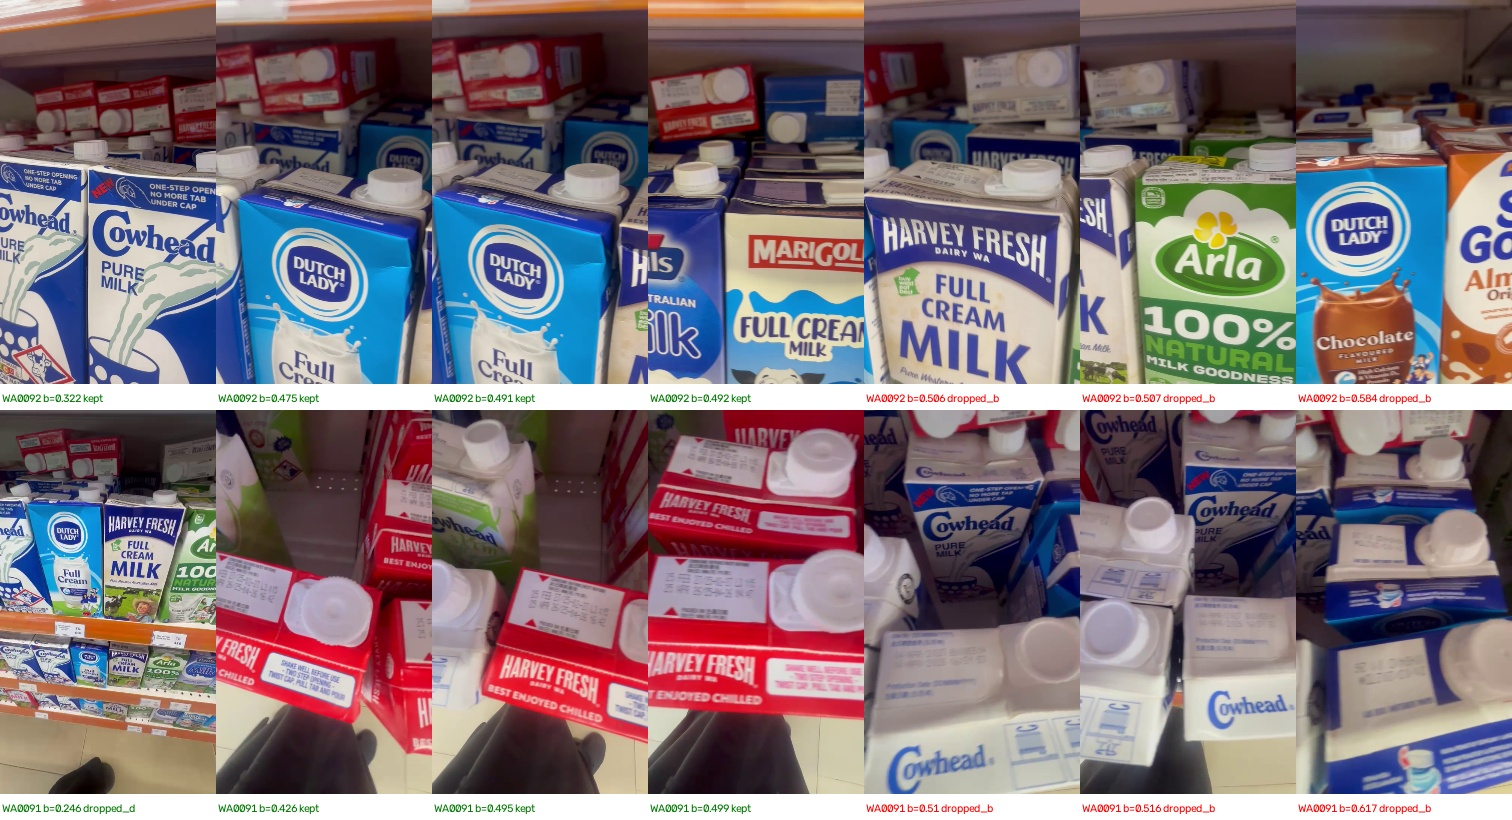
\includegraphics[width=\linewidth]{figures/blur_check.jpg}
\caption{Real motion blur in two milk-carton videos. Green: kept, red: dropped by the blur filter
(blur effect $b$ above 0.5).}
\label{fig:r4-blur}
\end{figure}

\subsubsection{Product detector}\label{sec:r4-det}
We trained YOLOv8n \cite{jocher2023yolov8,redmon2016yolo} with one class, \emph{product} (no
brands), on a random subset of SKU-110K \cite{goldman2019sku110k}: 2{,}000 training and 500
validation images. SKU-110K photos are up to about 4{,}000 pixels wide, so we shrank them once to
1{,}280 pixels to keep data loading fast. Training ran for 30 epochs at 1{,}024 pixels on a laptop
GTX~1650 (4\,GB) and took 163.5 minutes. Table~\ref{tab:r4-det} shows the validation results and
two settings that matter for dense shelves; Fig.~\ref{fig:r4-curves} shows the training curves.

\begin{table}[!t]
\centering
\caption{YOLOv8n on 500 SKU-110K validation images.}
\label{tab:r4-det}
\begin{tabular}{lcccc}
\hline
Setting & mAP50 & mAP50-95 & Precision & Recall \\
\hline
1{,}024\,px, max. 1{,}000 boxes (chosen) & \textbf{0.913} & \textbf{0.564} & 0.897 & 0.844 \\
1{,}024\,px, max. 299 boxes & 0.889 & 0.549 & 0.897 & 0.833 \\
640\,px, max. 1{,}000 boxes & 0.866 & 0.510 & 0.875 & 0.792 \\
\hline
\end{tabular}
\end{table}

\begin{figure}[!t]
\centering
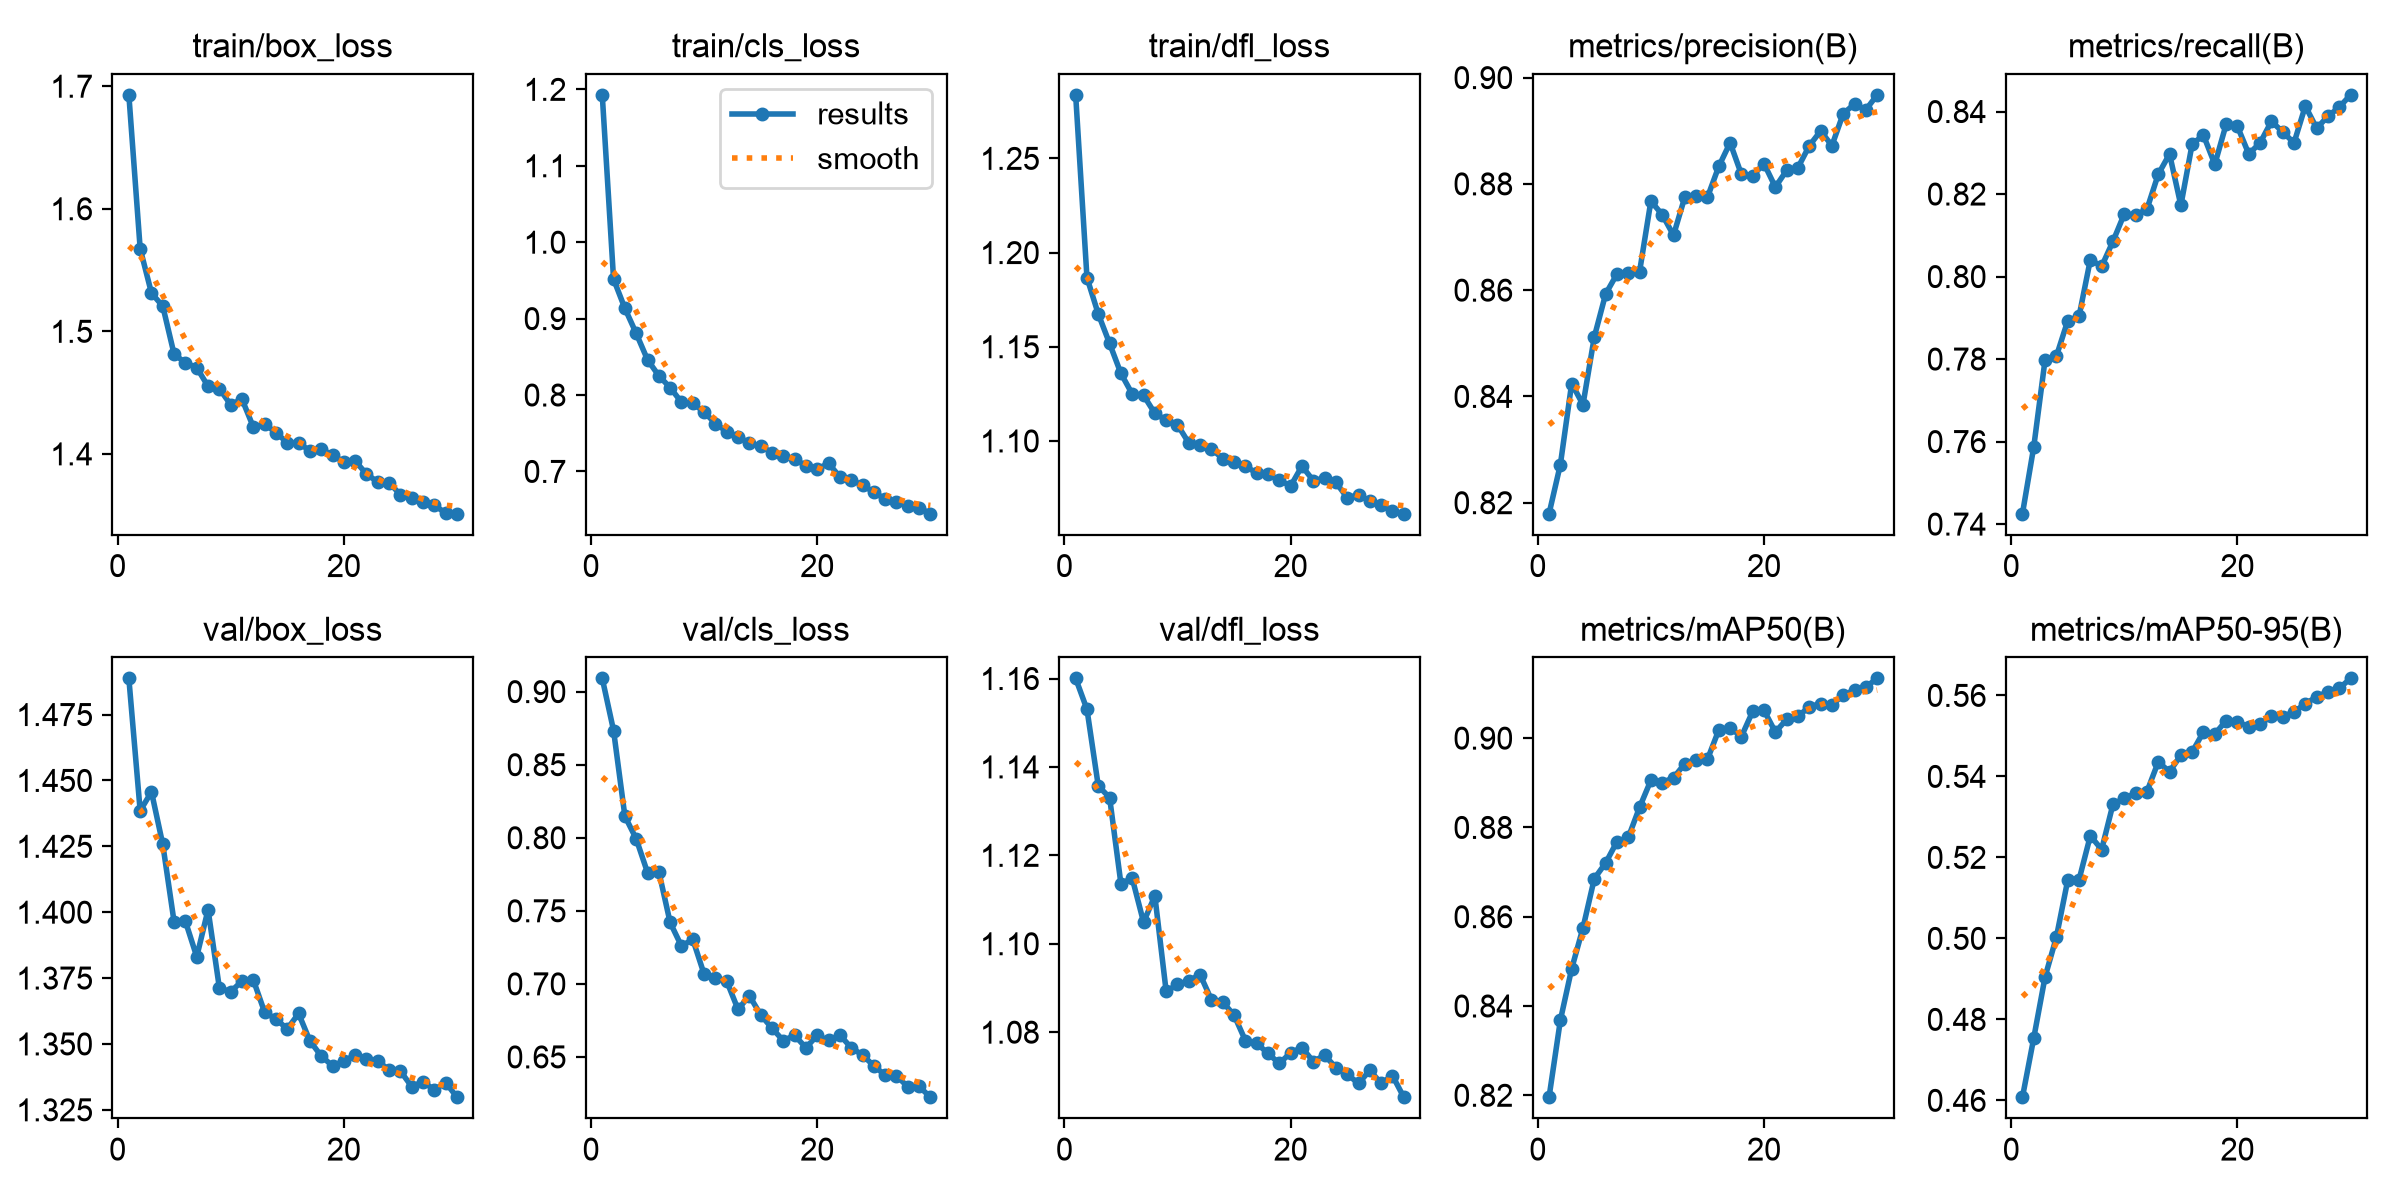
\includegraphics[width=\linewidth]{figures/sku110k_training_curves.png}
\caption{Training curves. Losses fall on both training and validation data, and mAP is still
rising at epoch 30.}
\label{fig:r4-curves}
\end{figure}

\begin{itemize}
  \item \textbf{Detection limit.} One validation image holds 718 products and 11 of 500 hold more
  than 300, so Ultralytics' default limit of 300 boxes per image costs 2.4 mAP50 points. We use
  1{,}000.
  \item \textbf{Image size.} Products are small, so the default 640\,px input costs 4.7 mAP50
  points against 1{,}024\,px.
  \item \textbf{On our footage.} The detector found 151{,}279 products on our 4{,}558 keyframes,
  a median of 29 per frame. It boxes nearly every item on packed shelves seen from a normal
  distance, but misses large products close to the camera (Fig.~\ref{fig:r4-detect}). Milk-carton
  close-ups get a median of 6 boxes per frame, against 53 for canned food, because SKU-110K
  products are small in the image.
  \item \textbf{mAP on our own frames} needs corrected labels and is carried over. The detector's
  boxes on the 222 annotation frames (median 30 per frame) are ready to be corrected in Roboflow,
  which is much faster than drawing every box.
\end{itemize}

\begin{figure}[!t]
\centering
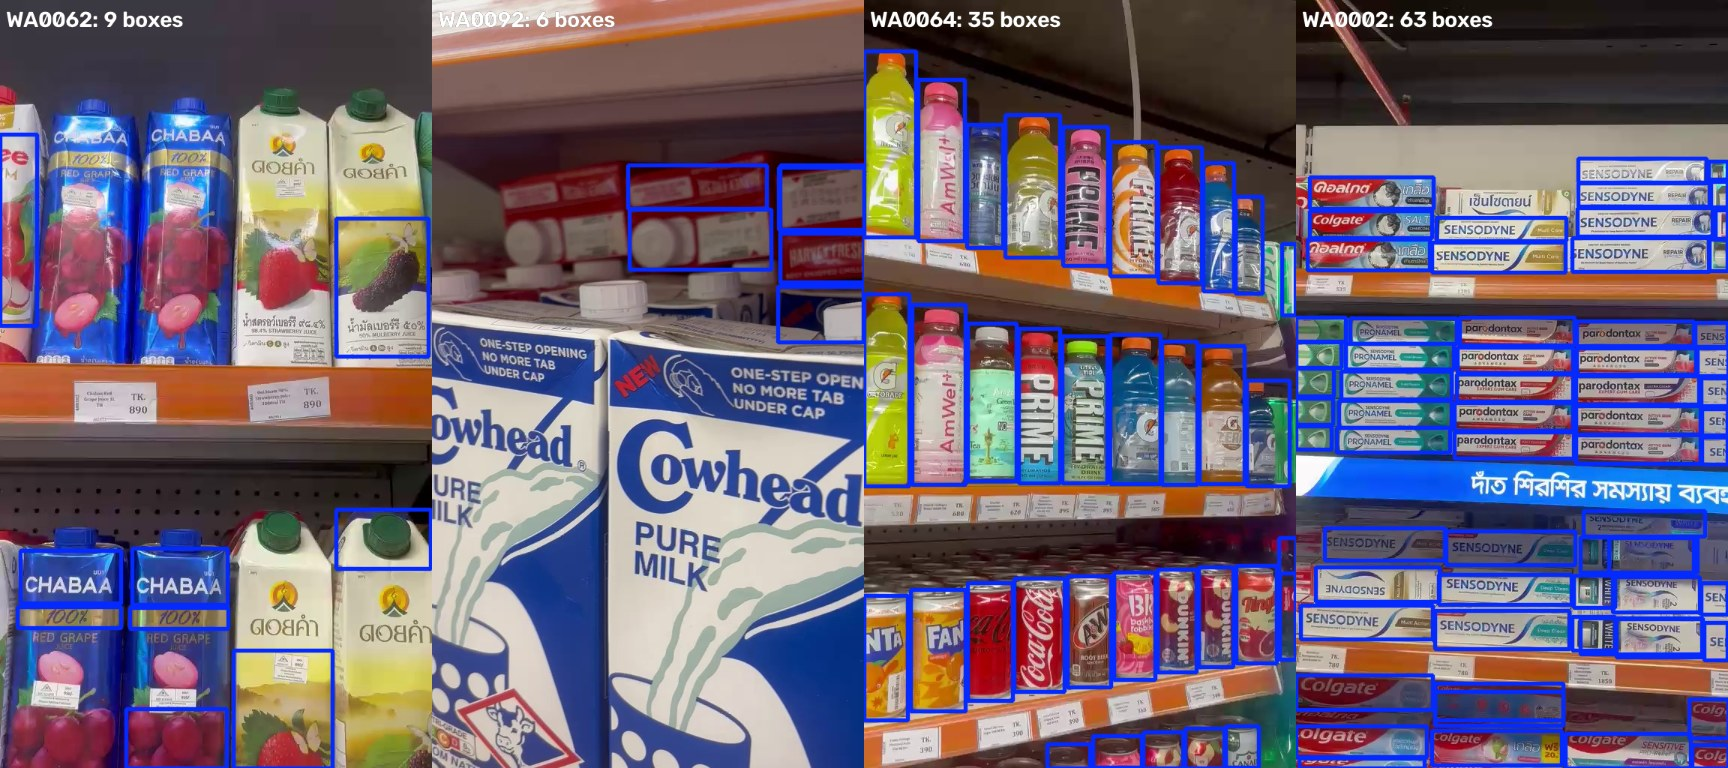
\includegraphics[width=\linewidth]{figures/detector_good_and_bad.jpg}
\caption{Detector output on our test videos. Left two: large close-up cartons are missed or split.
Right two: packed shelves at normal distance, where nearly every product is found.}
\label{fig:r4-detect}
\end{figure}

\subsubsection{Brand reading on product crops}\label{sec:r4-crops}
Report~3 concluded that the VLM should be asked about one product at a time. To test this we took
the 12 annotation frames of the six drinks-shelf test videos, cut 120 random detector crops, and
asked the same Qwen2-VL-2B model (fp16, zero-shot) ``which brand is this?'' for each crop and
``list the brands'' for each whole frame. Answers were matched to a catalogue of the 24 expected
brands, as an audit for a brand company would; the catalogue was built from our labels, so this is
an upper bound. Table~\ref{tab:r4-crops} shows the result and Fig.~\ref{fig:r4-crops} gives examples.

\begin{table}[!t]
\centering
\caption{Brand reading on 12 drinks-shelf frames: whole frame vs detector crops (Qwen2-VL-2B).}
\label{tab:r4-crops}
\begin{tabular}{lccc}
\hline
Method & Usable answers & Brand precision & Brand recall \\
\hline
Whole frame & 6 of 12 & 1.00 (6 frames) & 0.30 \\
Detector crops & 12 of 12 & 0.94 & \textbf{0.63} \\
\hline
\end{tabular}
\end{table}

\begin{figure}[!t]
\centering
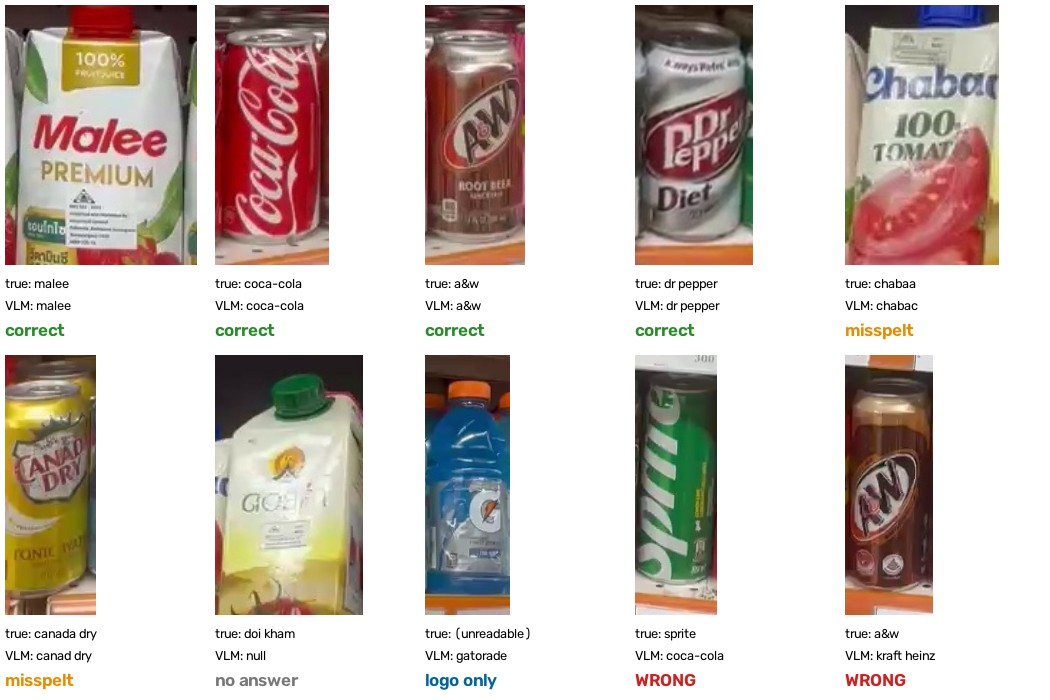
\includegraphics[width=\linewidth]{figures/crop_brand_examples.jpg}
\caption{Examples of single-product crops with the true brand and the VLM answer.}
\label{fig:r4-crops}
\end{figure}

\begin{itemize}
  \item Crops \textbf{doubled the brand recall} (0.30 $\rightarrow$ 0.63) at high precision. Six of
  the twelve whole-frame answers repeated words until the token limit and gave no usable list,
  the same loop seen in Report~3.
  \item Per crop, 48 of 67 readable crops were named correctly (72\%; 67\% before catalogue
  matching). Many raw answers are near-misses (``chabac'', ``canad dry'') that the catalogue fixes.
  \item Wrong brands are rare but biased: 2 of 120 crops were named ``Coca-Cola'' (for Canada Dry
  and Sprite), the same pull towards famous brands as in Report~3. A human must still check the
  evidence crop before a violation is reported.
  \item No answer was given for 11 readable crops, mostly brands written in Thai or Bengali script.
\end{itemize}
The crop and frame labels were drafted for this test and still need a second check by the team.

\subsubsection{Challenges faced}
\begin{itemize}
  \item \textbf{The new footage shows open shelves, not branded fridges.} It is ideal for product
  detection, share of shelf and price tags, but cooler purity still needs fridge recordings.
  \item \textbf{4\,GB of GPU memory.} A batch of 8 images at 1{,}024\,px needs 7.5\,GB and a batch of
  4 still overflowed on dense images, slowing training 2.7 times; we trained with batches of 2.
  Each data-loading worker also loaded its own copy of PyTorch, which exhausted Windows memory,
  so we used one worker.
  \item \textbf{A hidden default.} Ultralytics silently raises the 300-box limit during validation,
  which at first made our 300 vs 1{,}000 comparison meaningless; we re-measured with 299.
  \item \textbf{Licence.} SKU-110K may be used for academic, non-commercial work only and must not
  be redistributed, so its photos stay on our machine.
\end{itemize}

\subsubsection{Progress made}
Sprint~4 is mostly complete: the detector is trained and evaluated on SKU-110K, it runs on all our
keyframes, and the crop test supports the hybrid design. The remaining item is mAP on our own
frames, which needs the corrected labels.

\subsection{Target for next weekly update}
\begin{enumerate}
  \item Correct the pre-labels on the 222 keyframes in Roboflow, including empty-gap boxes; two
  members check every test frame.
  \item Fine-tune the detector on our 164 train frames and report mAP and counting error on our 58
  test frames.
  \item Verify the crop brand labels and the Sprint~3 ground truth.
  \item Record branded beverage fridges (15--30\,s each), including some with competitor products,
  to test cooler purity.
  \item Start Sprint~5: connect extraction, detection and the VLM into one pipeline that writes a
  JSON audit report with evidence (keyframe, timestamp, box) for every finding.
\end{enumerate}

\subsection{Individual contribution}
\begin{table}[!h]
\centering
\caption{Contribution summary.}
\begin{tabular}{lcc}
\hline
Task List & Member Assigned & Comments \\
\hline
Supermarket video recording & \TODO{member} & 115 videos \\
Video inventory, split and extraction & \TODO{member} & 4{,}558 keyframes \\
SKU-110K detector training and evaluation & \TODO{member} & mAP50 0.913 \\
Pre-labels and annotation frame selection & \TODO{member} & 222 frames \\
VLM crop test and brand labels & \TODO{member} & Recall 0.30 $\rightarrow$ 0.63 \\
\hline
\end{tabular}
\end{table}
